 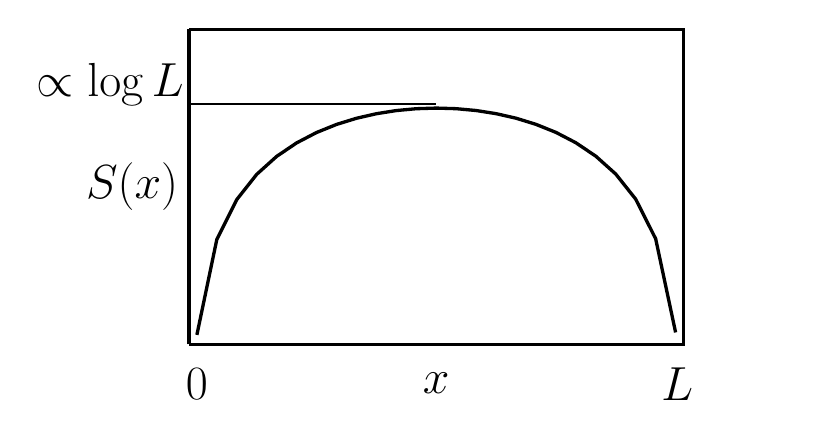
\begin{tikzpicture}[domain=0.1:6.18]
      \draw[very thick] (0, 0) -- (0,4) node[left, midway] {\LARGE $S(x)$} ;
       \node[] at (7.5, 2) {$$};
      \node[] at (3.14, -0.5){\LARGE $x$};
       \node[] at (-1, 3.3){\LARGE $\propto \log{L}$};
       \node[] at (0.1, -0.5){\LARGE $0$};
       \node[] at (6.2, -0.5){\LARGE $L$};
       \draw[thick] (0, 3.05) -- (3.14, 3.05);
      \draw[very thick] (0, 4)-- (6.28,4) -- (6.28, 0) -- (0, 0);
            \draw[color=black, very thick] plot (\x,{3+2/3*log2(sin(\x/2 r))}) node[right] {};
  \end{tikzpicture}